% Two-row hero composition for Fig. 1.
% Row 1: approved triptych (dry / SC window / bilayer hydrate) -- fig0_hero_boost.png
% Row 2: atom-resolved zoom of the bilayer-hydrate gallery -- fig0_hero_detail.png
% Thin gray "zoom" lines connect the third (bilayer-hydrate) scene of row 1
% to the full-width detail in row 2.  All labels live inside the artwork.
\documentclass[border=2pt]{standalone}
\usepackage{graphicx}
\usepackage{tikz}
\usetikzlibrary{calc}

\begin{document}
\begin{tikzpicture}
  % --- geometry ---
  \def\Wid{18cm}          % common width of both rows (equal pixel width => aligned)
  \def\Gap{0.30cm}        % vertical gap between the rows
  % fraction of row-1 width where the THIRD scene begins / ends
  \def\ThirdL{0.66}
  \def\ThirdR{1.00}

  % --- row 1 (top): the triptych ---
  \node[anchor=south west, inner sep=0] (r1)
        at (0,0) {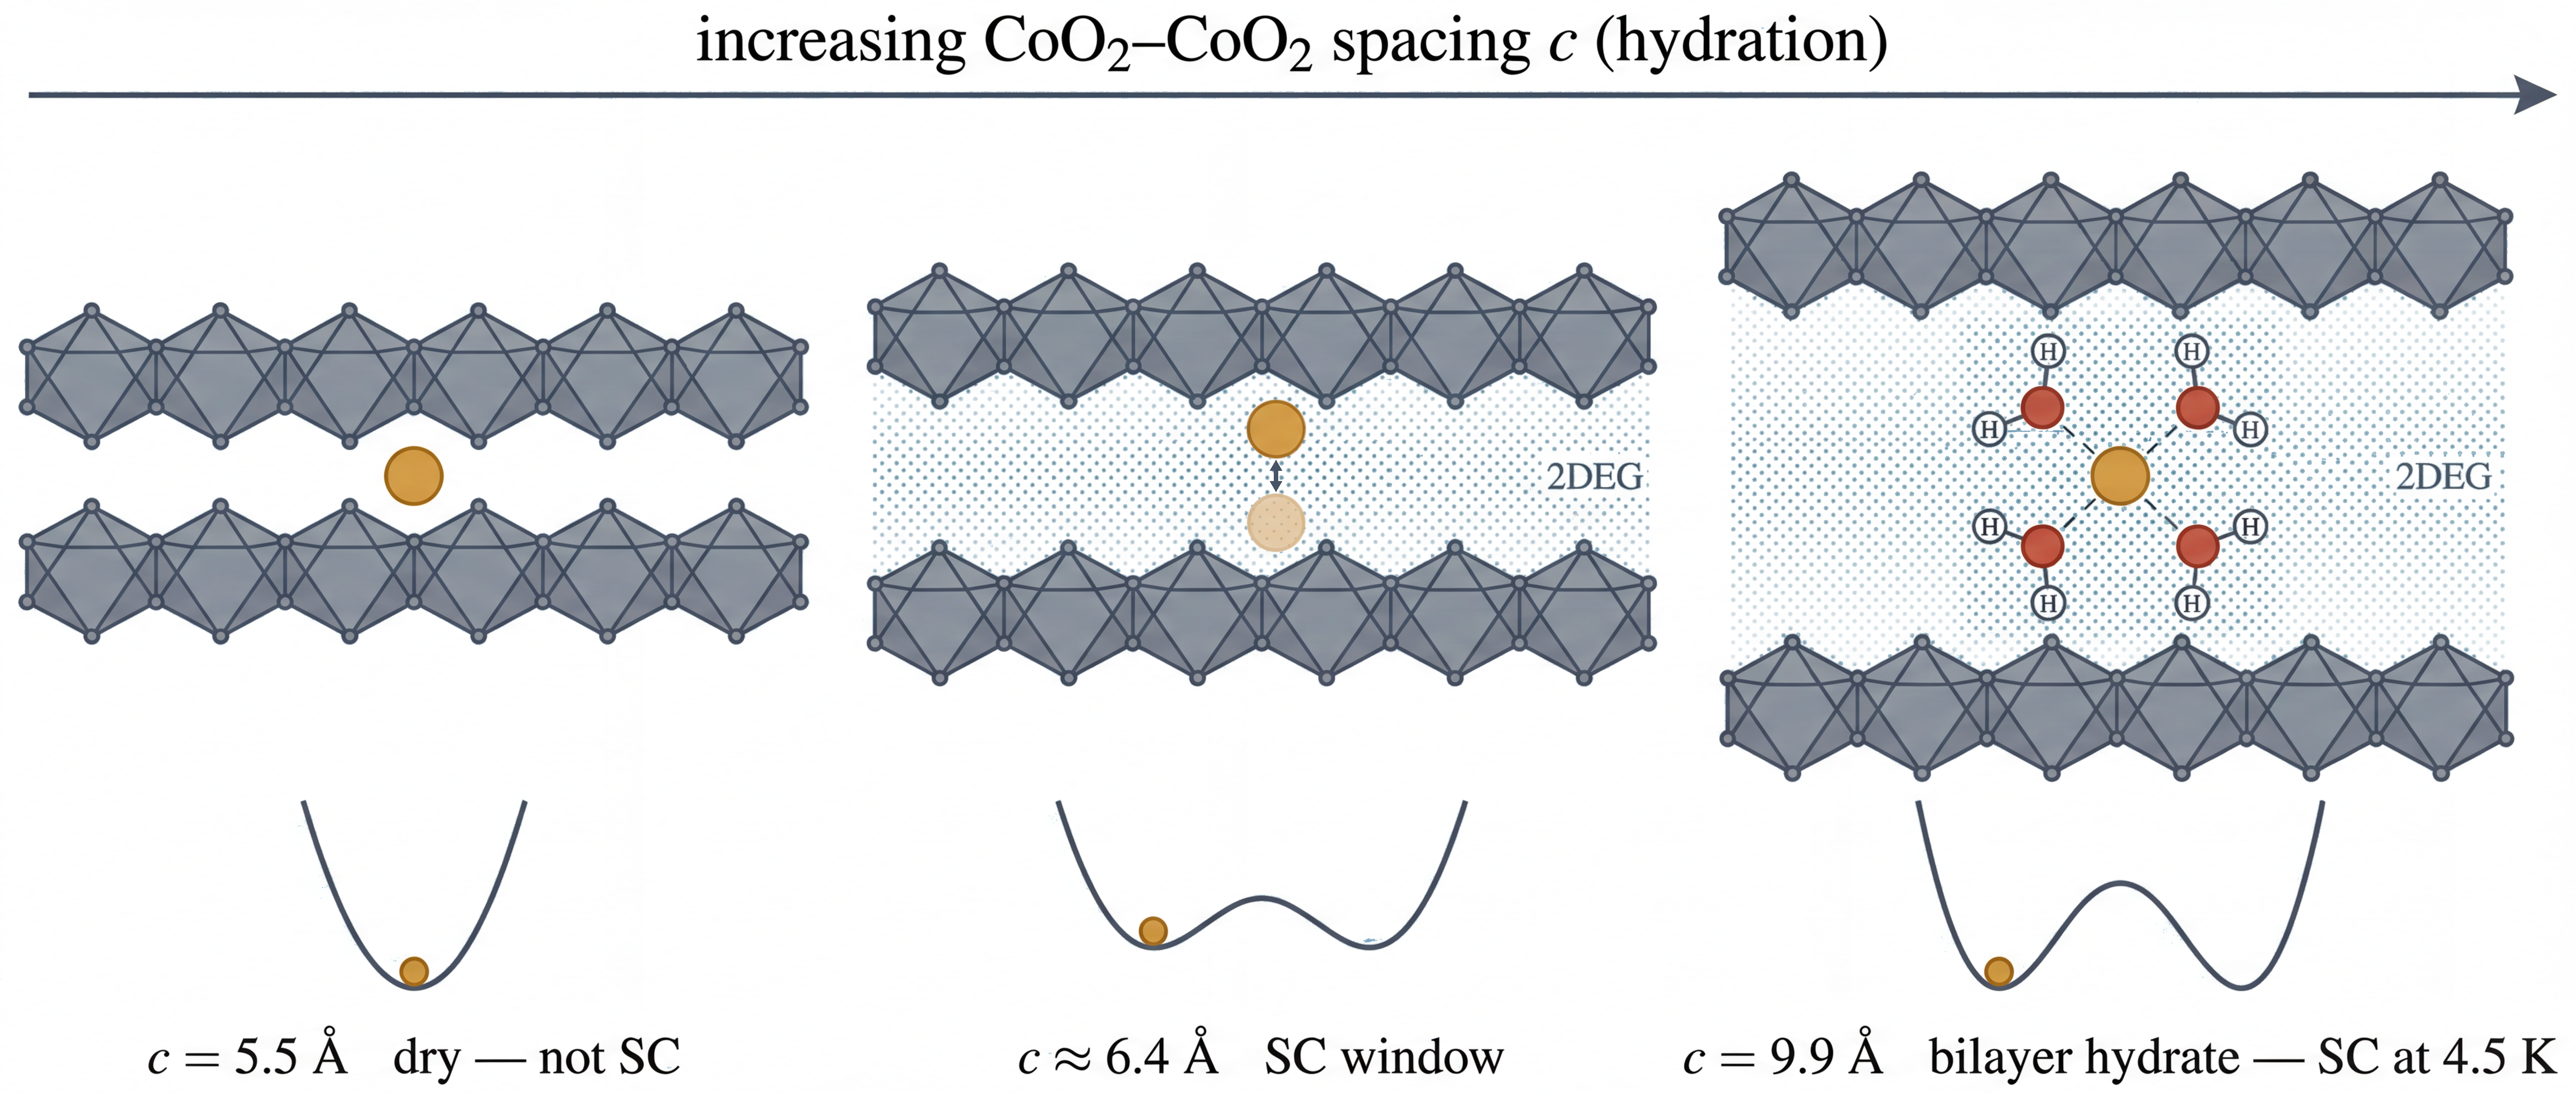
\includegraphics[width=\Wid]{../figures/fig0_hero_boost.png}};

  % --- row 2 (bottom): the atom-resolved zoom detail ---
  \node[anchor=north west, inner sep=0] (r2)
        at (0,-\Gap) {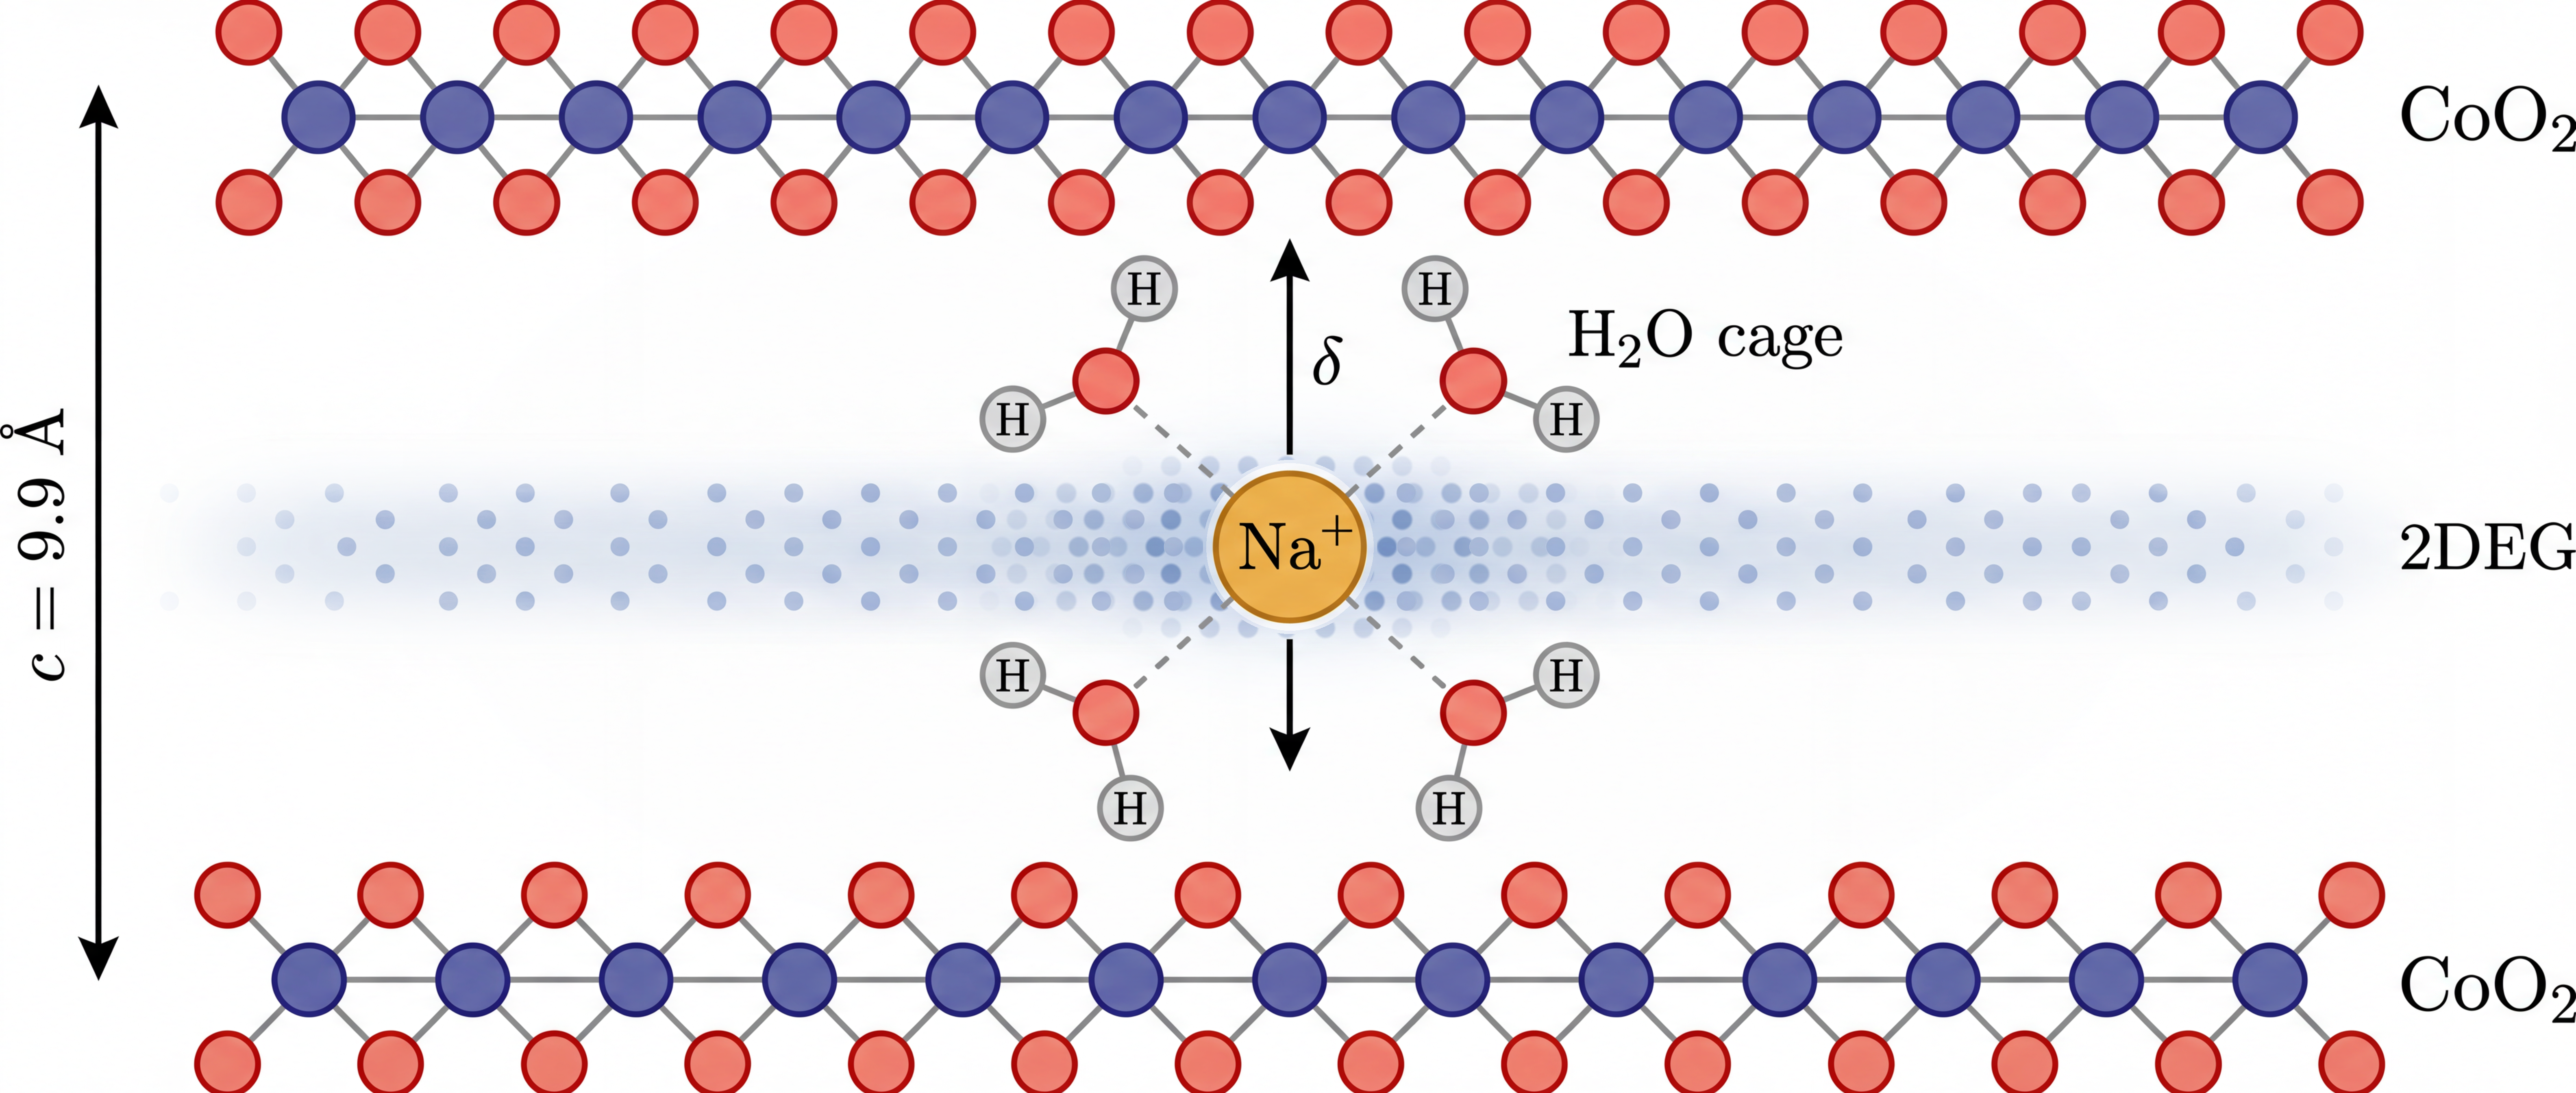
\includegraphics[width=\Wid]{../figures/fig0_hero_detail.png}};

  % source corners = bottom edge of the third scene of row 1
  \coordinate (sL) at ($(r1.south west)!\ThirdL!(r1.south east)$);
  \coordinate (sR) at ($(r1.south west)!\ThirdR!(r1.south east)$);

  % --- thin light-gray zoom lines fanning out to the full-width detail ---
  \draw[gray!45, line width=0.5pt] (sL) -- (r2.north west);
  \draw[gray!45, line width=0.5pt] (sR) -- (r2.north east);
\end{tikzpicture}
\end{document}
